\documentclass{article}
\usepackage[UTF8]{ctex}
\usepackage{tikz}
\usepackage{caption}
\usepackage{amsmath}
\usepackage{hyperref}
\usepackage{titlesec}
\usepackage{graphicx}
\usepackage[total={7in,10in}]{geometry}
\usepackage{subcaption}

\newcounter{para}
\newcommand\mypara{\par\refstepcounter{para}(\thepara)\space}
\titleformat{\section}[block]{\Large\bfseries\filcenter}{}{0em}{}
\renewcommand\thesection{}
\renewcommand\thesubsection{\setcounter{para}{0}\setcounter{equation}{0}第 \arabic{subsection} 题}

\usetikzlibrary{decorations.markings}

\title{hs\_phys\_probs 002}
\author{詹有丘}
\date{}

\begin{document}

\maketitle

\subsection{太空跳绳}
一根不可伸长的长度为 $l$, 质量为 $m$ 的均质软绳, 两端固定在间隔为 $b$ 的两点.
绳子以两个固定点的连线为轴以匀角速度 $\omega$ 转动.
忽略重力的影响而只考虑离心力.
转动过程中绳子的形状保持为一个平面图形不变.
(本题可以以积分及隐函数形式给出隐式解.)

\mypara
用平面坐标系中的方程描述绳子的形状.

\mypara
求绳子的动能.

\mypara
求固定点处对绳子的拉力的大小.

\subsection{地铁站闸机}
某地铁站的出入站闸机采用三锟闸设计.
三锟闸是这样一种装置:
考虑三维空间中的三根长度均为 $l$ 的细硬轻杆, 每根杆都有一端被固定在点 $O$ 处,
且它们两两之间的夹角被固定为 $\alpha$.
显然存在一条过 $O$ 的轴 $z$ 使得三锟闸绕 $z$ 轴有 $\frac{2\pi}3$ 旋转对称.
$z$ 轴与地面的夹角被适当地选取, 以至于三锟闸在初始状态可以与地面达成这样一种相对位形:
其中一根杆与地面平行, 另外两根杆的自由端的连线也与地面平行.
有一堵固定在地面上的墙, 其位置满足:
在初始状态下, 三锟闸的水平杆垂直于墙, 且墙面紧贴在水平杆的自由端.
将通过闸机的人简化为刚性长方体.
人通过闸机的过程中, 长方体推动三锟闸绕 $z$ 轴转动, 长方体的一个面紧贴地面, 另一个面紧贴墙面.
长方体足够高.

\mypara
求满足以下条件的长方体的最大宽度 $a_0$: 人能完全通过闸机, 且长方体的厚度可以任意大.

\mypara
接上问, 若长方体的宽度 $a>a_0$, 求满足以下条件的长方体的最大横截面积: 人能完全通过闸机.

\mypara
若长方体的宽度为 $a$, 人在完全通过闸机的过程中需要克服三种摩擦:
来自墙面和地面的滑动摩擦力 (大小恒定为 $f$),
来自杆的滑动摩擦力 (摩擦系数为 $\mu$),
来自三锟闸转轴的滑动摩擦力矩 (大小恒定为 $K$).
求人在缓慢地完全通过闸机的过程中, 来自杆的滑动摩擦耗散的能量为多少.

\subsection{Hohmann 转移轨道}
质量为 $m$ 的物体一开始绕着质量为 $M\gg m$ 的星体在半径为 $r_1$ 的圆轨道上运动.
某时其瞬间加速, 使速度方向不变, 速率增大 $\Delta v_1$, 进入椭圆轨道.
在远心点处, 其再次瞬间加速, 使速度方向不变, 速率增大 $\Delta v_2$,
进入半径为 $r_2=xr_1$ 的圆轨道上运动.
证明使 $\Delta v_1+\Delta v_2$ 最大的 $x$ 为
$5+4\sqrt7\cos\!\left(\frac13\arctan\frac{\sqrt3}{37}\right)$.

\subsection{电容势函数}
有一平行板电容器.
定义变量 $X$ 为极板间距, $Q$ 为一个极板上的电荷量大小,
$F$ 为极板间作用力, $V$ 为极板间的电势差.
电容 $C\!\left(X\right)$ 是已知函数 (不一定是反比例函数).
定义势函数 $U$ 为电容器储存的能量.

\mypara
证明 $\mathrm dU=V\,\mathrm dQ-F\,\mathrm dX$.

\mypara
证明 $\left(\frac{\partial V}{\partial F}\right)_Q=\left(\frac{\partial X}{\partial Q}\right)_F$.

\mypara
若 $C\!\left(X\right)$ 是反比例函数,
在 $F$-$X$ 图中分别作出等 $V$ 过程和等 $Q$ 过程的图像.

\subsection{张拉整体}
张拉整体 (tensegrity) 是一个由一些互不触碰的受压结构 (刚体) 以及连接它们的受拉结构 (绳) 组成的稳定结构.
其在建筑学, 工程学, 生物学等领域都有应用.
图 \ref{fig:张拉整体} (Cmglee, 2012) 是一个例子,
其由顶部和底部各一个边长为 $a$ 的正 $n$ 边形 (图中 $n=4$) 组成.
记底面的正 $n$ 边形为多边形 $\mathrm A_0\cdots\mathrm A_{n-1}$,
顶面上的正 $n$ 边形为多边形 $\mathrm B_0\cdots\mathrm B_{n-1}$.
$\mathrm A_0$ 与 $\mathrm A_n$ 是同一个点,
$\mathrm B_0$ 与 $\mathrm B_n$ 是同一个点.
对每个 $j$, 用长度为 $b$ 的轻绳连接 $\mathrm A_j\mathrm B_j$,
用长度为 $l$ 的轻杆连接 $\mathrm A_j\mathrm B_{j+1}$.

\mypara
多边形 $\mathrm A_0\cdots\mathrm A_{n-1}$ 在旋转一定角度 (旋转的方向与 $\mathrm A_j$ 随 $j$ 变化的环绕方向相同) 之后,
可以平移至与多边形 $\mathrm B_0\cdots\mathrm B_{n-1}$ 重合.
求该转角的最小正值.

\mypara
记 $T\!\left(\mathrm{PQ}\right)$ 为连接 $\mathrm P,\mathrm Q$ 两点的绳或杆上的力,
正值表示张力, 负值表示压力.
已知, 对每个 $j$, $T\!\left(\mathrm A_j\mathrm A_{j+1}\right)=T_0$.
对每个 $j$, 求 $T\!\left(\mathrm A_j\mathrm B_j\right)$ 和 $T\!\left(\mathrm A_j\mathrm B_{j+1}\right)$.

\begin{figure}[h!]
	\centering
	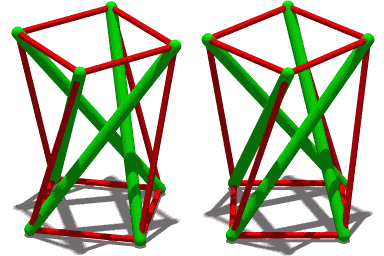
\includegraphics[width=0.5\linewidth]{Tensegrity_simple_4_RL.png}
	\caption{}
	\label{fig:张拉整体}
\end{figure}

\subsection{彩色视觉}

视觉感受器 (眼睛) 中对彩色视觉至关重要的生物基础是视锥细胞 (corn cell).
在光线充足的情况下, 视锥细胞比视杆细胞 (rod cell) 更加活跃,
我们因此不考虑视杆细胞对视觉带来的影响.
某种动物的视网膜上有 $n$ 种视锥细胞, 从而可以产生 $n$ 色视觉 ($n$-chromacy)
(人类有三色视觉 (trichromacy),
梅花雀有四色视觉 (tetrachromacy)\footnote{
	Hart N. S., Partridge J. C., Bennett A. T., Cuthill I. C.\@. ``Visual pigments, cone oil droplets and ocular media in four species of estrildid finch''. \textit{Journal of Comparative Physiology A}. Jul--Aug, 2000; \textbf{186} (7--8): 681--694. doi: 10.1007/s003590000121. PMID: 11016784. S2CID: 19458550.
},
青凤蝶 (\textit{Graphium sarpedon}) 有十五色视觉\footnote{
	Chen P., Awata H., Matsushita A., Yang E., Arikawa K.\@. ``Extreme Spectral Richness in the Eye of the Common Bluebottle Butterfly, \textit{Graphium sarpedon}''. \textit{Frontiers in Ecology and Evolution}, vol. 4, pp. 18. Mar 8, 2016. doi: 10.3389/fevo.2016.00018. ISSN: 2296-701X.
}).
第 $j$ 种视锥细胞对波长为 $\lambda$ 的光的吸收率为 $f_j\!\left(\lambda\right)$,
其中 $f_j$ 看作 $\mathbf f:\left(0,+\infty\right)\to$ 的第 $j$ 个分量.
第 $j$ 种视锥细胞在某种光刺激下的响应程度正比于它从中吸收的总功率.
视锥细胞在受到刺激后, 会将响应信号以电信号的形式告诉大脑,
大脑即可获得视网膜上某处的各种视锥细胞的响应程度 $\mathbf c\in\left[0,+\infty\right)^n$,
其中 $\mathbf c$ 的分量 $c_j$ 为第 $j$ 种视锥细胞的响应程度.
从而颜色可以与 $C:=\left[0,+\infty\right)^n$ 中的向量一一对应.

规定两种变换: $T_u:c_j\mapsto uc_j$ ($u>0$)
以及 $S_v:c_j\mapsto v\left(c_j-l\right)+l$ ($0<v\le\frac l{c_{\min}}$),
其中 $l$ 是 $\mathbf c$ 中最小分量 $c_{\min}$ 和最大分量 $c_{\max}$ 的平均值.
我们认为在这两种变换下 $\mathbf c$ 的色相保持不变.
我们关于色相建立一个等价关系: $\mathbf c\sim\mathbf c'$
当且仅当存在 $u,v$, 使得 $\mathbf c=T_uS_v\mathbf c'$.

设某种设备 (不妨称为彩灯) 能发出固定的 $n$ 种单色光, 其波长分别为 $\lambda_k$.
它能以任意不同的功率合成并发出这些单色光, 产生对视锥细胞的光刺激.

彩虹中包含了所有的单色光.

\mypara
设某个光刺激中能量随波长的分布为已知函数 $g\!\left(\lambda\right)$,
求该光刺激代表的颜色.

\mypara
求彩灯能产生的所有的颜色的集合 $L\subseteq C$.

\mypara
求彩虹中所有的颜色的集合 $R\subseteq C$.

\mypara
若存在一组 $\left\{\lambda_k\right\}$, 使得 $L=C$.
求 $f_j$ 需要满足的条件.

\mypara
是否对于任意的 $\mathbf c\in C$, 存在 $\mathbf c'\in R$, 使得 $\mathbf c\sim\mathbf c'$?
若是, 给出构造 $\mathbf c'$ 的方法.
若否, 是否对于几乎所有的 $\mathbf c\in C$, 不存在这样的 $\mathbf c'$?

\mypara
是否对于任意的 $\mathbf c\in C$, 存在 $\mathbf c'\in L$, 使得 $\mathbf c\sim\mathbf c'$?
若是, 给出构造 $\mathbf c'$ 的方法.
若否, 是否对于任意的 $\mathbf c\in R$, 存在 $\mathbf c'\in L$, 使得 $\mathbf c\sim\mathbf c'$?

\subsection{互 LC 震荡}

我们知道电感有自感和互感.
但是, 虽然我们有``互电容''的概念, 其并不能与互感很好地对应.
我们现在来构造一种与互感相对应的概念``互容'':
考虑四块的面积为 $S$ 的平行极板, 依次编号为 a--d.
极板 a 和极板 c 看作一个电容器, 极板间距为 $d_1$;
极板 b 和极板 d 看作一个电容器, 极板间距为 $d_2$;
极板 b 和极板 c 的间距为 $d$.

\mypara
求这两个电容器之间的互容系数.

\mypara
设有两个 LC 电路,
电路中分别有电容 $C_1$ 与 $C_2$, 电感 $L_1$ 与 $L_2$.
两个电容之间的互容系数为 $N$, 两个电感之间的互感系数为 $M$.
设在 $t=0$ 时两个电容分别带电 $Q_{10}$ 与 $Q_{20}$,
求任意时刻 $t$ 时两个电容所带的电荷量 $Q_1\!\left(t\right)$ 与 $Q_2\!\left(t\right)$.

\subsection{球套黑球}

本题中提到的黑体都是余弦辐射体.
将一个热容为 $C$ 的半径为 $r$ 的均匀的球形的黑体 A
放在一个半径为 $R$ 的均匀的薄球壳 B 内.
两个球心的距离为 $d<R-r$.
在 $t=0$ 时, A 的温度为 $T_0$.
A 内部的热传导很快.

\mypara
B 是热容为 $D$, 初始温度为 $S_0$ 的黑体.
求 $t$ 时刻 A 的温度 $T\!\left(t\right)$.

\mypara
B 的内壁是可以完全反射热辐射的镜面.
求 $t$ 时刻 A 的温度 $T\!\left(t\right)$.

\newpage
\section{参考答案}

\subsection{太空跳绳}

\mypara
因为绳子的形状是具有最小势能的形状, 所以本题即求解最优化问题
\begin{alignat}{2}
	\min_{y\in C^1\left[-b/2,b/2\right]}\quad & \int_{-b/2}^{b/2}-\frac12\cdot\frac ml\sqrt{1+y'^2}\,\mathrm dx\cdot\omega^2\cdot y^2\\
	\mathrm{s.t.}\quad & y\!\left(-b/2\right)=y\!\left(b/2\right)=0,\\
	& \int_{-b/2}^{b/2}\sqrt{1+y'^2}\,\mathrm dx=l.
	\label{eq:绳长约束}
\end{alignat}
在目标函数中带上 Lagrange 乘子, 可以略去约束条件式 \ref{eq:绳长约束}, 而目标变为
\begin{alignat}{2}
	\max_{y\in C^1\left[-b/2,b/2\right]}\quad & \int_{-b/2}^{b/2}y^2\sqrt{1+y'^2}\,\mathrm dx-\lambda\left(\int_{-b/2}^{b/2}\sqrt{1+y'^2}\,\mathrm dx-l\right)\\
	\mathrm{s.t.}\quad & y\!\left(-b/2\right)=y\!\left(b/2\right)=0.
\end{alignat}

定义 Lagrangian
\begin{equation}
	\mathcal L:=\left(y^2-\lambda\right)\sqrt{1+y'^2}.
\end{equation}
代入 Euler--Lagrange 方程后化简可得
\begin{equation}
	2y\left(1+y'^2\right)=\left(y^2-\lambda\right)y''.
\end{equation}
进行变换 $p:=y'$ 后可得
\begin{equation}
	2y\left(1+p^2\right)=\left(y^2-\lambda\right)p\frac{\mathrm dp}{\mathrm dy}.
\end{equation}
分离变量并积分可得
\begin{equation}
	\ln\!\left(1+p^2\right)=2\ln\frac{a^2-y^2}{a^2-y_0^2},
	\label{eq:变分法}
\end{equation}
其中 $y_0:=y\!\left(0\right)>0$, $a:=\sqrt\lambda>y_0$.
回代 $p=y'$, 再次分离变量并积分可得
\begin{equation}
	\int_{y_0}^y\frac{\mathrm dy}{\sqrt{\left(\frac{a^2-y^2}{a^2-y_0^2}\right)^2-1}}=\pm x.
	\label{eq:曲线方程}
\end{equation}
式 \ref{eq:曲线方程} 给出描述绳子形状的方程.

约束条件 $y\!\left(-b/2\right)=y\!\left(b/2\right)=0$ 给出
\begin{equation}
	b=2\int_0^{y_0}\frac{\mathrm dy}{\sqrt{\left(\frac{a^2-y^2}{a^2-y_0^2}\right)^2-1}}.
	\label{eq:b约束}
\end{equation}
绳子上的长度微元
\begin{equation}
	\mathrm ds=\sqrt{1+y'^2}\,\mathrm dx=\frac{a^2-y^2}{a^2-y_0^2}\frac{\mathrm dy}{\sqrt{\left(\frac{a^2-y^2}{a^2-y_0^2}\right)^2-1}}=\frac{\mathrm dy}{\sqrt{1-\left(\frac{a^2-y_0^2}{a^2-y^2}\right)^2}}.
\end{equation}
从而
\begin{equation}
	l=2\int_0^{y_0}\frac{\mathrm dy}{\sqrt{1-\left(\frac{a^2-y_0^2}{a^2-y^2}\right)^2}}.
	\label{eq:l约束}
\end{equation}
式 \ref{eq:b约束} 与式 \ref{eq:l约束} 隐式给出了式 \ref{eq:曲线方程} 中的参数 $a$ 和 $y_0$.

\mypara
\begin{equation}
	E_\mathrm k=\int_{x=-b/2}^{b/2}\frac12\cdot\frac ml\,\mathrm ds\cdot \omega^2y^2=\frac{m\omega^2}{l}\int_0^{y_0}\frac{y^2\,\mathrm dy}{\sqrt{1-\left(\frac{a^2-y_0^2}{a^2-y^2}\right)^2}}.
\end{equation}

\mypara
质心位置为
\begin{equation}
	y_\mathrm c=\frac1m\int_{x=-b/2}^{b/2}y\cdot\frac ml\,\mathrm ds
	=\frac2l\int_0^{y_0}\frac{y\,\mathrm dy}{\sqrt{1-\left(\frac{a^2-y_0^2}{a^2-y^2}\right)^2}}=\frac{y_0\sqrt{2a^2-y_0^2}}l.
\end{equation}
绳子受到的合力
\begin{equation}
	F=m\omega^2y_\mathrm c
	=\frac{m\omega^2y_0\sqrt{2a^2-y_0^2}}l.
\end{equation}

在 $x=\pm b/2$ 处曲线的切线斜率
\begin{equation}
	y'\!\left(\pm b/2\right)=\mp\tan\theta=\mp\sqrt{\left(\frac{a^2}{a^2-y_0^2}\right)^2-1},
\end{equation}
从而固定点处对绳子的拉力大小
\begin{equation}
	T_{\pm b/2}=\frac F{2\sin\theta}
	=\frac{m\omega^2y_0\sqrt{2a^2-y_0^2}}{2l\sqrt{1-\left(\frac{a^2-y_0^2}{a^2}\right)^2}}
	=\frac{m\omega^2a}{2l}.
\end{equation}

\textit{另}: 此题可用受力法解.

\begin{figure}[h!]
	\centering
	\begin{tikzpicture}
		\draw[thick,->] (-1,0) -- (5,0) node[anchor=north] {$x$};
		\draw[thick,->] (0,-1) -- (0,5) node[anchor=east] {$y$};
		\draw[domain=0:2,smooth,variable=\x] plot ({\x}, {4-\x*\x/2});
		\draw[thick,->] (0,4) node[anchor=north east] {$y_0$} -- (-0.7,4) node[anchor=east] {$T_0$};
		\draw[thick,->] (1,3.5) -- (1,4.9) node[anchor=west] {$\int_0^x\frac ml\,\mathrm ds\cdot\omega^2\cdot y$};
		\draw[dashed] (2,2) node[anchor=north west] {$\theta$} -- (3,2);
		\draw[thick,->] (2,2) -- (2.7,0.6) node[anchor=west] {$T$};
	\end{tikzpicture}
	\caption{}
	\label{fig:绳子受力分析}
\end{figure}

设绳子在 $x=0$ 处的张力为水平方向 $T_0$,
考虑 $\left[0,x\right]$ 上的一段绳子的受力平衡, 如图 \ref{fig:绳子受力分析} 所示.
考虑到 $\tan\theta=-y'$, 有
\begin{equation}
	\int_0^x\frac ml\,\mathrm ds\cdot\omega^2\cdot y=-T_0y'.
\end{equation}
两边对 $x$ 求导可得
\begin{equation}
	\frac{m\omega^2}{l}\sqrt{1+y'^2}=-T_0y''.
\end{equation}
变换 $p:=y'$, 分离变量得
\begin{equation}
	\frac{p\,\mathrm dp}{\sqrt{1+p^2}}=-\frac{m\omega^2}{T_0l}y\,\mathrm dy.
\end{equation}
两边积分得
\begin{equation}
	\sqrt{1+p^2}-1=-\frac{m\omega^2}{2T_0l}\left(y^2-y_0^2\right).
	\label{eq:受力法}
\end{equation}
代换 $a:=\sqrt{\frac{2T_0l}{m\omega^2}+y_0^2}$ 可将式 \ref{eq:受力法} 变为与式 \ref{eq:变分法} 等价的形式.

\subsection{地铁站闸机}

\subsection{Hohmann 转移轨道}

物体的速度变化的全过程为
\begin{equation}
	\underbrace{\sqrt{\frac{GM}{r_1}}}_{\text{圆轨道}}\xrightarrow{\Delta v_1}
	\underbrace{\sqrt{-\frac{2GM}{r_1+r_2}+\frac{2GM}{r_1}}
	\rightarrow\sqrt{-\frac{2GM}{r_1+r_2}+\frac{2GM}{r_2}}}_{\text{椭圆轨道}}
	\xrightarrow{\Delta v_2}\underbrace{\sqrt{\frac{GM}{r_2}}}_{\text{圆轨道}}.
\end{equation}

于是
\begin{equation}
	\Delta v_1+\Delta v_2\propto f\!\left(x\right):=\sqrt{\frac{2x}{1+x}}-1+\sqrt{\frac1x}-\sqrt{\frac2{x\left(1+x\right)}}.
\end{equation}
为了使 $\Delta v_1+\Delta v_2$ 极大,
\begin{equation}
	f'\!\left(x\right)=-\frac12x^{-\frac32}-\frac1{\sqrt2}x^{-\frac12}\left(1+x\right)^{-\frac32}+\frac1{\sqrt2}\left(1+2x\right)x^{-\frac32}\left(1+x\right)^{-\frac32}=0.
	\label{eq:f'(x)=0}
\end{equation}
在式 \ref{eq:f'(x)=0} 两边乘 $2x^{\frac32}\left(1+x\right)^{\frac32}$ 可得
\begin{equation}
	\sqrt2\left(1+3x\right)-\left(1+x\right)^{\frac32}=0.
\end{equation}
此方程可约化为多项式方程
\begin{equation}
	P\!\left(x\right):=x^3-15x^2-9x-1=0.
\end{equation}

注意到
\begin{equation*}
	\cos3y=\cos y\left(2\cos^2y-1\right)-2\cos y\left(1-\cos^2y\right)=4\cos^3y-3\cos y,
\end{equation*}
所以
\begin{equation*}
	\cos^3\frac y3=\frac14\left(\cos y+3\cos\frac y3\right).
\end{equation*}

令 $x^\star:=5+4\sqrt7\cos\!\left(\frac13\arctan\frac{\sqrt3}{37}\right)$, 则
\begin{align}
	\left(x^\star-5\right)^3&=16\cdot 7^{\frac 32}\left(\cos\arctan\frac{\sqrt3}{37}+3\cos\!\left(\frac13\arctan\frac{\sqrt3}{37}\right)\right)\\
	&=16\cdot 7^{\frac 32}\left(\frac{37}{2\cdot 7^{\frac32}}+3\cdot\frac{x^\star-5}{4\sqrt7}\right)\\
	&=84x^\star-124.
\end{align}
由此可得 $P\!\left(x^\star\right)=0$.

\subsection{电容势函数}

\mypara
$V\,\mathrm dQ$ 是电源对电容所做的功, $-F\,\mathrm dX$ 是外力对电容所做的功.

\mypara
令 $H:=U+FX$, 则
\begin{equation}
	\mathrm dH=V\,\mathrm dQ+X\,\mathrm dF.
\end{equation}
从而
\begin{equation}
	V=\left(\frac{\partial H}{\partial Q}\right)_F,\qquad X=\left(\frac{\partial H}{\partial F}\right)_Q.
\end{equation}
由于求偏导次序可交换,
$\frac{\partial^2H}{\partial Q\partial F}=\frac{\partial^2H}{\partial F\partial Q}$,
因此
\begin{equation}
	\left(\frac{\partial V}{\partial F}\right)_Q=\left(\frac{\partial X}{\partial Q}\right)_F.
\end{equation}

\mypara
设 $C\!\left(X\right)=\alpha/X$, 则由 $Q=CV$ 可得状态方程
\begin{equation}
	QX=\alpha V.
\end{equation}
内能表达式为
\begin{equation}
	U=\frac12QV=\frac{Q^2X}{2\alpha}.
\end{equation}
于是
\begin{equation}
	F=-\left(\frac{\partial U}{\partial X}\right)_Q=\frac{Q^2}{2\alpha}=\frac{\alpha V^2}{2X^2}.
\end{equation}
于是可以在 $F$-$X$ 图作出如图 \ref{fig:电容势函数的图} 所示的曲线.
图 \ref{fig:等V过程} 与图 \ref{fig:等Q过程} 分别是等 $V$ 过程与等 $Q$ 过程的图像.

\begin{figure}[h!]
	\centering
	\begin{subfigure}[b]{0.4\linewidth}
		\centering
		\begin{tikzpicture}
			\draw[thick,->] (0,0) -- (5,0) node[anchor=north] {$X$};
			\draw[thick,->] (0,0) -- (0,4) node[anchor=east] {$F$};
			\draw[domain=0.9:4.5,smooth,variable=\x] plot ({\x},{3/\x/\x});
		\end{tikzpicture}
		\caption{等 $V$ 过程}
		\label{fig:等V过程}
	\end{subfigure}
	\begin{subfigure}[b]{0.4\linewidth}
		\centering
		\begin{tikzpicture}
			\draw[thick,->] (0,0) -- (5,0) node[anchor=north] {$X$};
			\draw[thick,->] (0,0) -- (0,4) node[anchor=east] {$F$};
			\draw (0.5,2.5) -- (4.5,2.5);
		\end{tikzpicture}
		\caption{等 $Q$ 过程}
		\label{fig:等Q过程}
	\end{subfigure}
	\caption{}
	\label{fig:电容势函数的图}
\end{figure}

\subsection{张拉整体}

\subsection{彩色视觉}

\subsection{互 LC 震荡}

\subsection{球套黑球}

\end{document}
